In this section we detail our reference scenario for MRS coordination and as well 
as the formalization of the problem we addressed and the solutions we propose.

\section{Problem description}
Our reference scenario is based on a warehouse that stores items of various types.
Such items must be composed together to satisfy orders that arrive based on customers’ demand.
The items of various types are stored in particular sections of the building (\textit{loading bay})
and must be trasported to a set of \textit{unloading bays} where such items are then 
packed together by human operators. The set of items to be trasported and where they should
go depends on the orders.

In our domain a set of robots is responsible for transporting items from
the loading bay to the unloading bays and the system goal is to maximize the
throughput of the orders, i.e., to maximize the number of orders completed in
the unit of time. Now, robots involved in transportation tasks move around
the warehouse and are likely to interfere when they move in close proximity,
and this can become a major source of inefficiency (e.g., robots must slow down
and they might even collide causing serious delays in the system).
Hence, a crucial aspect to maintain highly efficient and safe operations is to minimize the
possible spatial interferences between robots.

The main goal of our system is composing simple tasks to create a subset of complex tasks
to improve the productivity and minimize the robot's time travel and the paths distance.

To manage the merging of the task we can use a range of different techniques. 
In the setion \ref{solution} there are the strategies used to create subsets of tasks. 
After the composing step, we have varieties of tasks subsets. At the end to validate which is the best
subset we propose an heuristic. This heuristic function normalize the overall path of the subset of tasks
based on the number of items that each robot can carry.
Furthermore the purpose is to maximize the number of items in the same journey.


\section{Problem fomalization}
In this section we formalize the MRS coordination problem described above as a task allocation problem
where the robots must be allocated to transportation tasks. 

In our formalization we have a finite set of tasks. A robot can execute a task if it is available else the robot will go at start position.
For how the system is built, a robot to request a task must arrive at the previous vertex of the loading bay.

In more detail, our model considers a set of items of different types $E = \{ e_1,...,e_N\}$,
stored in a specific loading bay ($L$). The warehouse must serve a set of orders 
$O=\{o_1,...,o_M\}$. Orders are processed in one or more than one of the unloading bays ($U_i$).
Each order is defined by a vector of demand for each item type (the number of required 
items to close the order). Hence, $o_j = < d_{1,j},...,d_{N,j}>$, where $d_{i,j}$ is the 
demand for order $j$ of items of type $i$. When an order is finished a new one arrives,
until the set of task is finished.
The orders induce a set of $N \times M$ trasportation tasks $T = {t_{i,j}}$, with 
$t_{i,j} = < d_{i,j}, P_{i,j}>$, where $t_{i,j}$ defines the task of transporting 
$d_{i,j}$ items of type $i$ for order $o_j$ (hence to unloading bay $U_j$).
Each task has a destination bay for centralized coordination the $t_{i,j}$ has a set of edges
$P_{i,j}$ which respects the strategy used. 
We have a set of robot $R = \{r_1,...,r_K \}$ that can execute transportation tasks, where
each robot has a defined load capacity for each item type $C_k = <c_{1,k},...,c_{N,k}>$, 
hence $c_{i,k}$ is the load capacity of robot $k$ for items of type $i$.

We consider in our logistic scenario, homogenous robots, which have the same radius 
and the same capacity. Because often in the logistic environments robots are all 
equal. 

% formalizzare la euristica
Since the main of this thesis is composing subsets of tasks we formalize what is 
a subset of tasks and what we mean for merging paths of a subset of tasks and 
which is the heuristic funcion used for differentiate the subests of tasks or simple tasks.

Specifically given a set of tasks $\mathcal{T}$ it define intrinsically a set of orders $O$.
One order perform a subset of $\mathcal{T}$. A subest of tasks $S$, denoted by $S\subseteq\mathcal{T}$.

Where $S = \{T_1,\cdots,T_k\}$ for each element of the subset we combine their paths $P$ to form a single path $\pi$.
For $\pi$ define a path that perform the travel order such as a vector of vertices $\pi = \{v_1,\cdots,v_i\}$.
% figure dell'unione di due path

\begin{figure}[hbt]
    \begin{multicols}{2}
        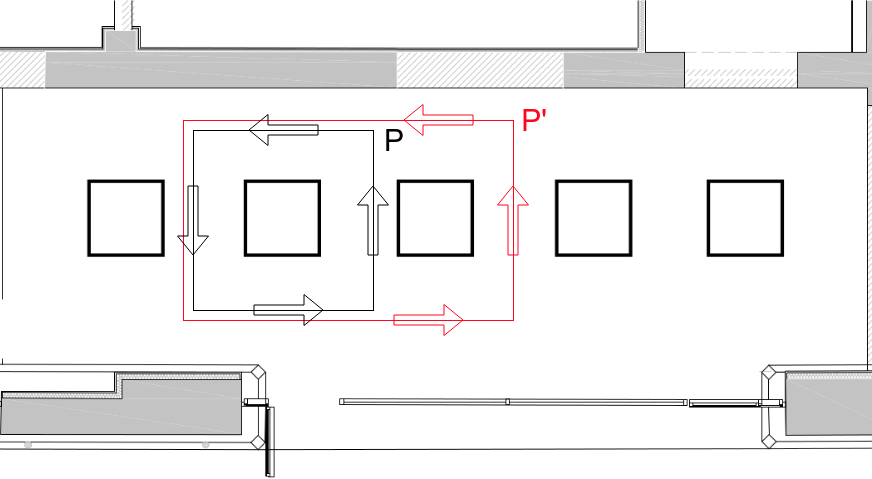
\includegraphics[width=\linewidth]{img/p1p2_cut.png}
        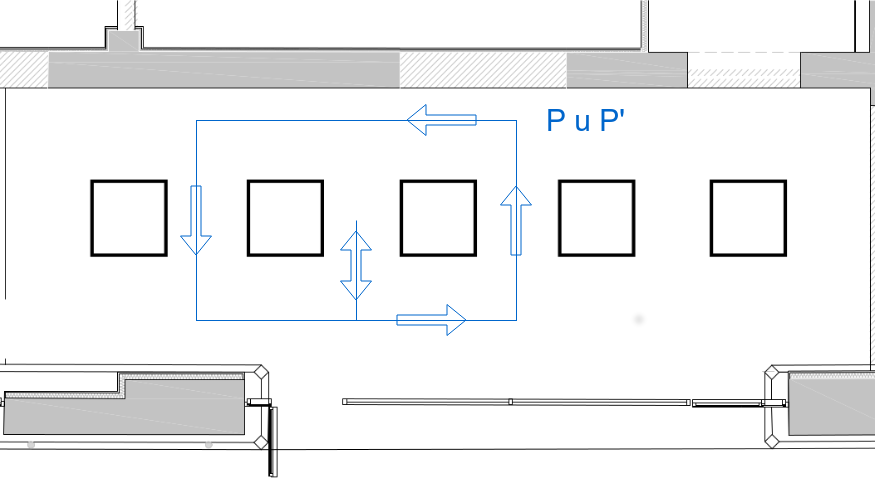
\includegraphics[width=\linewidth]{img/p3_cut.png}
    \end{multicols}
    \caption{Comparison of the union of two paths $P$ and $P'$ to form a single path $\pi = P \cup P'$.}
\end{figure}

% funzione che calcola il percorso distaza

The function $p(\cdot)$ is used to join the paths, this funcion return the vector of vertices $\pi$. 

For calculate the cost of the paths we used a function $f(\cdot)$ that return the path distance.

Because we maximize the total demand ($d_S$) we calculate the sum the single demand for each element in the subset.
More formally:
\[d_S =demand(T_1) + \cdots + demand(T_k)\]

where $demand(\cdot)$ return the single demand of the specific task.

Another function used in our system is $dst(\cdot)$ that return the euclidean distances between loading and unloading bays.

Finally we define our heuristic function $v(\cdot)$ which
can be defined for any task $T$ or subsets $S$:
\[ v(T) = \frac{f(P)}{demand(T)}\]

This heuristic function is used for normalize the cost of path (path distance) 
on the demand (cost of the item/items) of the order. 

For compute the best partition of tasks the heuristic is based on the concept of loss $L$,
which can be defined for any pair of subset $S_i$, $S_j$ as:
\[L(S_i,S_j) = v(\{ S_i \cup S_j\}) - v(S_i) - v(S_j)\]
where $v(S)$ is value of the characteristic function $v(\cdot)$ for subset $S$.
In other worlds, this loss funcion captures the value of synergies between subsets
and is computed in constant time. 

The function $v$ for a subset $S$ is defined as:
\[ v(S) = \frac{f(\pi)}{d_S}\]
where $f(\pi)$ is the path distance between the loading bay $L$ and the unloading bays $U_j$ and the distance
to return to the initial vertex and the $d_s$ is the total demand of the tasks.

We want minimize the cost of the loss, that can be defined as:
\[L(S_i,S_j) < 0 \]
if the loss $L$ is less than 0 then we allocate the pair and delete the element which
form the subset.







